\section{Extras}\label{sec:extras}
\mkAgenda

\subsection{Errors}\label{subsec:errors}
\begin{frame}[fragile]{Errors}
    \center
    \begin{itemize}
        \item<1-> CUDA functions return \CUDA{cudaError_t}, useful with \CUDA{cudaGetErrorString()}
    \end{itemize}
\begin{minted}[breaklines=true]{CUDA}
#define CHECK(x) do { \
    const auto _ = (x); \
    if(_ != cudaSuccess) { \
        /* ... handle error using cudaGetErrorString(_) */\
    } \
} while(false)
\end{minted}
\end{frame}

\subsection{Memory}\label{subsec:memory}
\begin{frame}{Memory}
    \center
    \begin{itemize}
        \item Manage GPU memory
        \item Allocate with \CUDA{cudaMalloc(void **dev, size_t bytes)}
        \item Read/Write CPU-side with \CUDA{cudaMemcpy(void *dst, const void *src, size_t bytes, cudaMemcpyKind kind)}
        \begin{itemize}
            \item \CUDA{cudaMemcpyDefault}: Inferred based on pointers (CUDA 4+)
            \item \CUDA{cudaMemcpyHostToDevice}: CPU \textrightarrow GPU
            \item \CUDA{cudaMemcpyDeviceToHost}: GPU \textrightarrow CPU
            \item \CUDA{cudaMemcpyDeviceToDevice}: GPU \textrightarrow GPU
            \item \CUDA{cudaMemcpyHostToHost}: CPU \textrightarrow CPU
        \end{itemize}
        \item Unified Memory: \CUDA{cudaMallocManaged(void **dev, size_t bytes)} (accessible on CPU \& GPU)
        \item Free/Clean up with \CUDA{cudaFree(void *dev)}
    \end{itemize}
\end{frame}

\subsection{Synchronization}\label{subsec:synchronization}
\begin{frame}[fragile]{Synchronization}
    \center
    \begin{itemize}
        \item Atomic functions like \CUDA{atomicAdd}
        \item Across threads/warps in block: \CUDA{__syncthreads()}
        \item Make CPU wait for GPU: \CUDA{cudaDeviceSynchronize()}
        \item More advanced:
        \begin{itemize}
            \item Selected threads using \CUDA{cuda::barrier}
            \item All threads across blocks: \CUDA{this_grid().sync()} (requires Cooperative Groups and launch using \CUDA{cudaLaunchCooperativeKernel})
        \end{itemize}
    \end{itemize}
\end{frame}

\subsection{CUDA and OpenGL}\label{subsec:cuda-opengl}
\begin{frame}[t]{CUDA and OpenGL}
    \begin{columns}
        \begin{column}{0.5\textwidth}
            \centerline{
\includegraphics[height=2cm]{./figures/cuda}}
            \begin{itemize}
                \item High-performance GPU compute
            \end{itemize}
        \end{column}
        \begin{column}{0.5\textwidth}
            \centerline{
\includegraphics[height=2cm]{./figures/opengl}}
            \begin{itemize}
                \item Real-time 3D graphics
            \end{itemize}
        \end{column}
    \end{columns}
    \centerline{If both are on the same GPU, they can communicate!}
    \begin{itemize}
        \item CUDA can read from/write to OpenGL buffers
        \item OpenGL will use the updated data to render
        \item That all without using the CPU or any extensive memory copying
    \end{itemize}
\end{frame}

\begin{frame}{CUDA and OpenGL}
    \centerline{\resizebox{0.95\linewidth}{!}{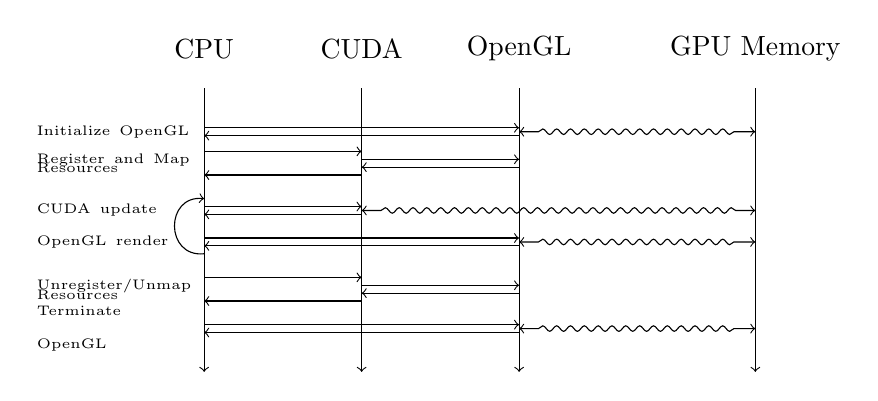
\begin{tikzpicture}[decoration = {snake,pre length=7pt,post length=7pt,amplitude=1pt,segment length=5pt}]
    % Arrows/timelines
    \draw[->] (0,0) -- (0,-3.6);
    \draw (0,0.5) node[anchor=center] {CPU};
    \draw[->] (2,0) -- (2,-3.6);
    \draw (2,0.5) node[anchor=center] {CUDA};
    \draw[->] (4,0) -- (4,-3.6);
    \draw (4,0.5) node[anchor=center] {OpenGL};
    \draw[->] (7,0) -- (7,-3.6);
    \draw (7,0.5) node[anchor=center] {GPU Memory};

    % Steps
    \draw[->] (0, -0.5) -- (4, -0.5);
    \draw[<->,decorate] (4, -0.55) -- (7, -0.55);
    \draw[<-] (0, -0.6) -- (4, -0.6);
    \draw (0, -0.55) node[anchor=east,text width=2cm] {{\tiny Initialize OpenGL}};

    \draw[->] (0, -0.8) -- (2, -0.8);
    \draw[->] (2, -0.9) -- (4, -0.9);
    \draw[<-] (2, -1.0) -- (4, -1.0);
    \draw[<-] (0, -1.1) -- (2, -1.1);
    \draw (0, -0.95) node[anchor=east,text width=2cm] {\shortstack[l]{\tiny Register and Map\\[-4pt]\tiny Resources}};

    \draw[->] (0, -1.5) -- (2, -1.5);
    \draw[<->,decorate] (2, -1.55) -- (7, -1.55);
    \draw[<-] (0, -1.6) -- (2, -1.6);
    \draw (0, -1.55) node[anchor=east,text width=2cm] {{\tiny CUDA update}};

    \draw[->] (0, -1.9) -- (4, -1.9);
    \draw[<->,decorate] (4, -1.95) -- (7, -1.95);
    \draw[<-] (0, -2.0) -- (4, -2.0);
    \draw (0, -1.95) node[anchor=east,text width=2cm] {{\tiny OpenGL render}};

    \draw[->] (0, -2.1) .. controls (-0.5,-2.15) and (-0.5,-1.35) .. (0, -1.4);

    \draw[->] (0, -2.4) -- (2, -2.4);
    \draw[->] (2, -2.5) -- (4, -2.5);
    \draw[<-] (2, -2.6) -- (4, -2.6);
    \draw[<-] (0, -2.7) -- (2, -2.7);
    \draw (0, -2.55) node[anchor=east,text width=2cm] {\shortstack[l]{\tiny Unregister/Unmap\\[-4pt]\tiny Resources}};

    \draw[->] (0, -3.0) -- (4, -3.0);
    \draw[<->,decorate] (4, -3.05) -- (7, -3.05);
    \draw[<-] (0, -3.1) -- (4, -3.1);
    \draw (0, -3.05) node[anchor=east,text width=2cm] {{\tiny Terminate OpenGL}};
\end{tikzpicture}}}
\end{frame}

\begin{frame}[fragile]{CUDA and OpenGL}
    \center
    \begin{itemize}
        \item<1-> \CUDA{__device__} functions can access OpenGL data
    \end{itemize}
    \begin{minted}[breaklines=true]{CUDA}
#include <cuda_gl_interop.h>
// set up on CPU
cudaGraphicsResource *resource; T *dev_ptr; size_t size;
cudaGraphicsGLRegisterBuffer(&resource, handle, cudaGraphicsRegisterFlagsNone);
cudaGraphicsMapResources(1, &resource);
cudaGraphicsResourceGetMappedPointer(
    reinterpret_cast<void **>(&dev_ptr), &size, resource
);
// ... do stuff with dev_ptr on GPU
// clean up on CPU
cudaGraphicsUnmapResources(1, &resource);
cudaGraphicsUnregisterResource(resource);
    \end{minted}
\end{frame}